%----------------------------------------------------------------------------------------
%       DOCUMENT CONFIGURATION AND INCLUDED PACKAGES
%----------------------------------------------------------------------------------------

\documentclass[english, 10pt,a4paper,oneside,headinclude,footinclude,BCOR5mm]{scrartcl}
\usepackage[nochapters, beramono, eulermath, pdfspacing, dottedtoc ]{classicthesis}

\usepackage{arsclassica}
\usepackage[T1]{fontenc} 
\usepackage[utf8]{inputenc}

\usepackage{graphicx}
\usepackage{tcolorbox}
\usepackage{subfig}
\usepackage{mathtools}
\usepackage{subcaption}
\usepackage{pgfplots}
\usepackage{wrapfig}
\usepackage{tikz}
\usepackage{circuitikz}
\usepackage{siunitx}
\usepackage{tikz-3dplot}
\graphicspath{{figures/}}

\usepackage{enumitem}
\usepackage{lipsum}
\usepackage{varioref}
\usepackage{csquotes}
\usepackage{cancel}

\usepackage{amsmath,amssymb,amsthm}
\usepackage{xfrac}
\usepackage{braket}
\usepackage{upgreek}
\usepackage[version=4]{mhchem}
\usepackage{eulervm}

\usepackage[numbers,sort&compress]{natbib}
\bibliographystyle{unsrtnat}

\hypersetup{
%draft, % Uncomment to remove all links (useful for printing in black and white)
colorlinks=true, breaklinks=true, bookmarks=true,bookmarksnumbered,
urlcolor=webbrown, linkcolor=RoyalBlue, citecolor=webgreen,
pdftitle={},
pdfauthor={\textcopyright},
pdfsubject={},
pdfkeywords={},
pdfcreator={pdfLaTeX},
pdfproducer={LaTeX with hyperref and ClassicThesis}
}


\newtheoremstyle{mytheorem}% Name
  {\topsep}   % Space above
  {\topsep}   % Space below
  {\itshape}  % Body font
  {}          % Indent amount
  {\bfseries} % Head font
  {:}         % Punctuation after theorem head
  {.5em}      % Space after theorem head
  {\thmname{#1}\thmnote{\ (\textbf{#2})}}          % Theorem head spec
\theoremstyle{mytheorem}
\newtheorem{satz}{Satz}[section]


\usepackage[a4paper, margin=2.5cm]{geometry}


\usepackage[english]{babel}

\begin{document}

%----------------------------------------------------------------------------------------
%	CONFIGURE HEADERS, TITLEPAGE, TABLE OF CONTENTS
%----------------------------------------------------------------------------------------
\renewcommand{\sectionmark}[1]{\markright{\spacedlowsmallcaps{#1}}} 
\lehead{\mbox{\llap{\small\thepage\kern1em\color{halfgray} \vline}\color{halfgray}\hspace{0.5em}\rightmark\hfil}} 
\pagestyle{plain} 


\begin{center}
    \large Advanced Computational Physics, University of Strathclyde, WS 2026,\\ Dr. Ben Hourahine

    \vspace{0.5cm}

    {\LARGE\bfseries Assignment 4\par}

    \vspace{0.5cm}

    \large Jörn Wilhelm\\
    Glasgow, 21.\ April 2026

    \vspace{1cm}
\end{center}

\newcommand{\cancelblue}[2]{
  \textcolor{blue}{\cancelto{#1}{\textcolor{black}{#2}}}
}
\newcommand{\overblue}[2]{
  \textcolor{blue}{\overbrace{\textcolor{black}{#2}}^{#1}}
}
\newcommand{\underblue}[2]{
  \textcolor{blue}{\underbrace{\textcolor{black}{#2}}_{#1}}
}
\newcommand{\blue}[1]{\textcolor{blue}{#1}}
\newcommand{\red}[1]{\textcolor{red}{#1}}
%----------------------------------------------------------------------------------------
%	ACTUAL CONTENT
%----------------------------------------------------------------------------------------

\section{Ising model}
\subsection{Metropolis}
The results of applying the standard Metropolis scheme to the Ising model are shown in 
Figure \ref{fig:ising-metropolis} for lattices of size $L=16,64,256,1024$\,. We expect a phase transition of second order to happen at the 
critical temperature $T_c=2/\ln(1+\sqrt{2})\approx 2.269$\,. Thus, the system should be 
in the ordered state for $T<T_c$\,, i.e. $M/L^2=1$\,, and the linear response
$C_V$ should diverge at $T=T_c$\,. Due to considering a finite system,
the specific heat does not diverge but spike. For $L=16$ such could be observed.
For larger lattices, the algorithm did not fully converge in 
$16\cdot1000\cdot L^2$. Reason for this is that each Metropolis step only flips one spin, making
it almost impossible to reach the fully ordered state in reasonable time.
This issue will be adressed later on. An immediate fix would be to intialize the lattice in the ordered state, however
this will break down for $T>T_c$ and the XY model.
\begin{figure}[h!]
  \centering
  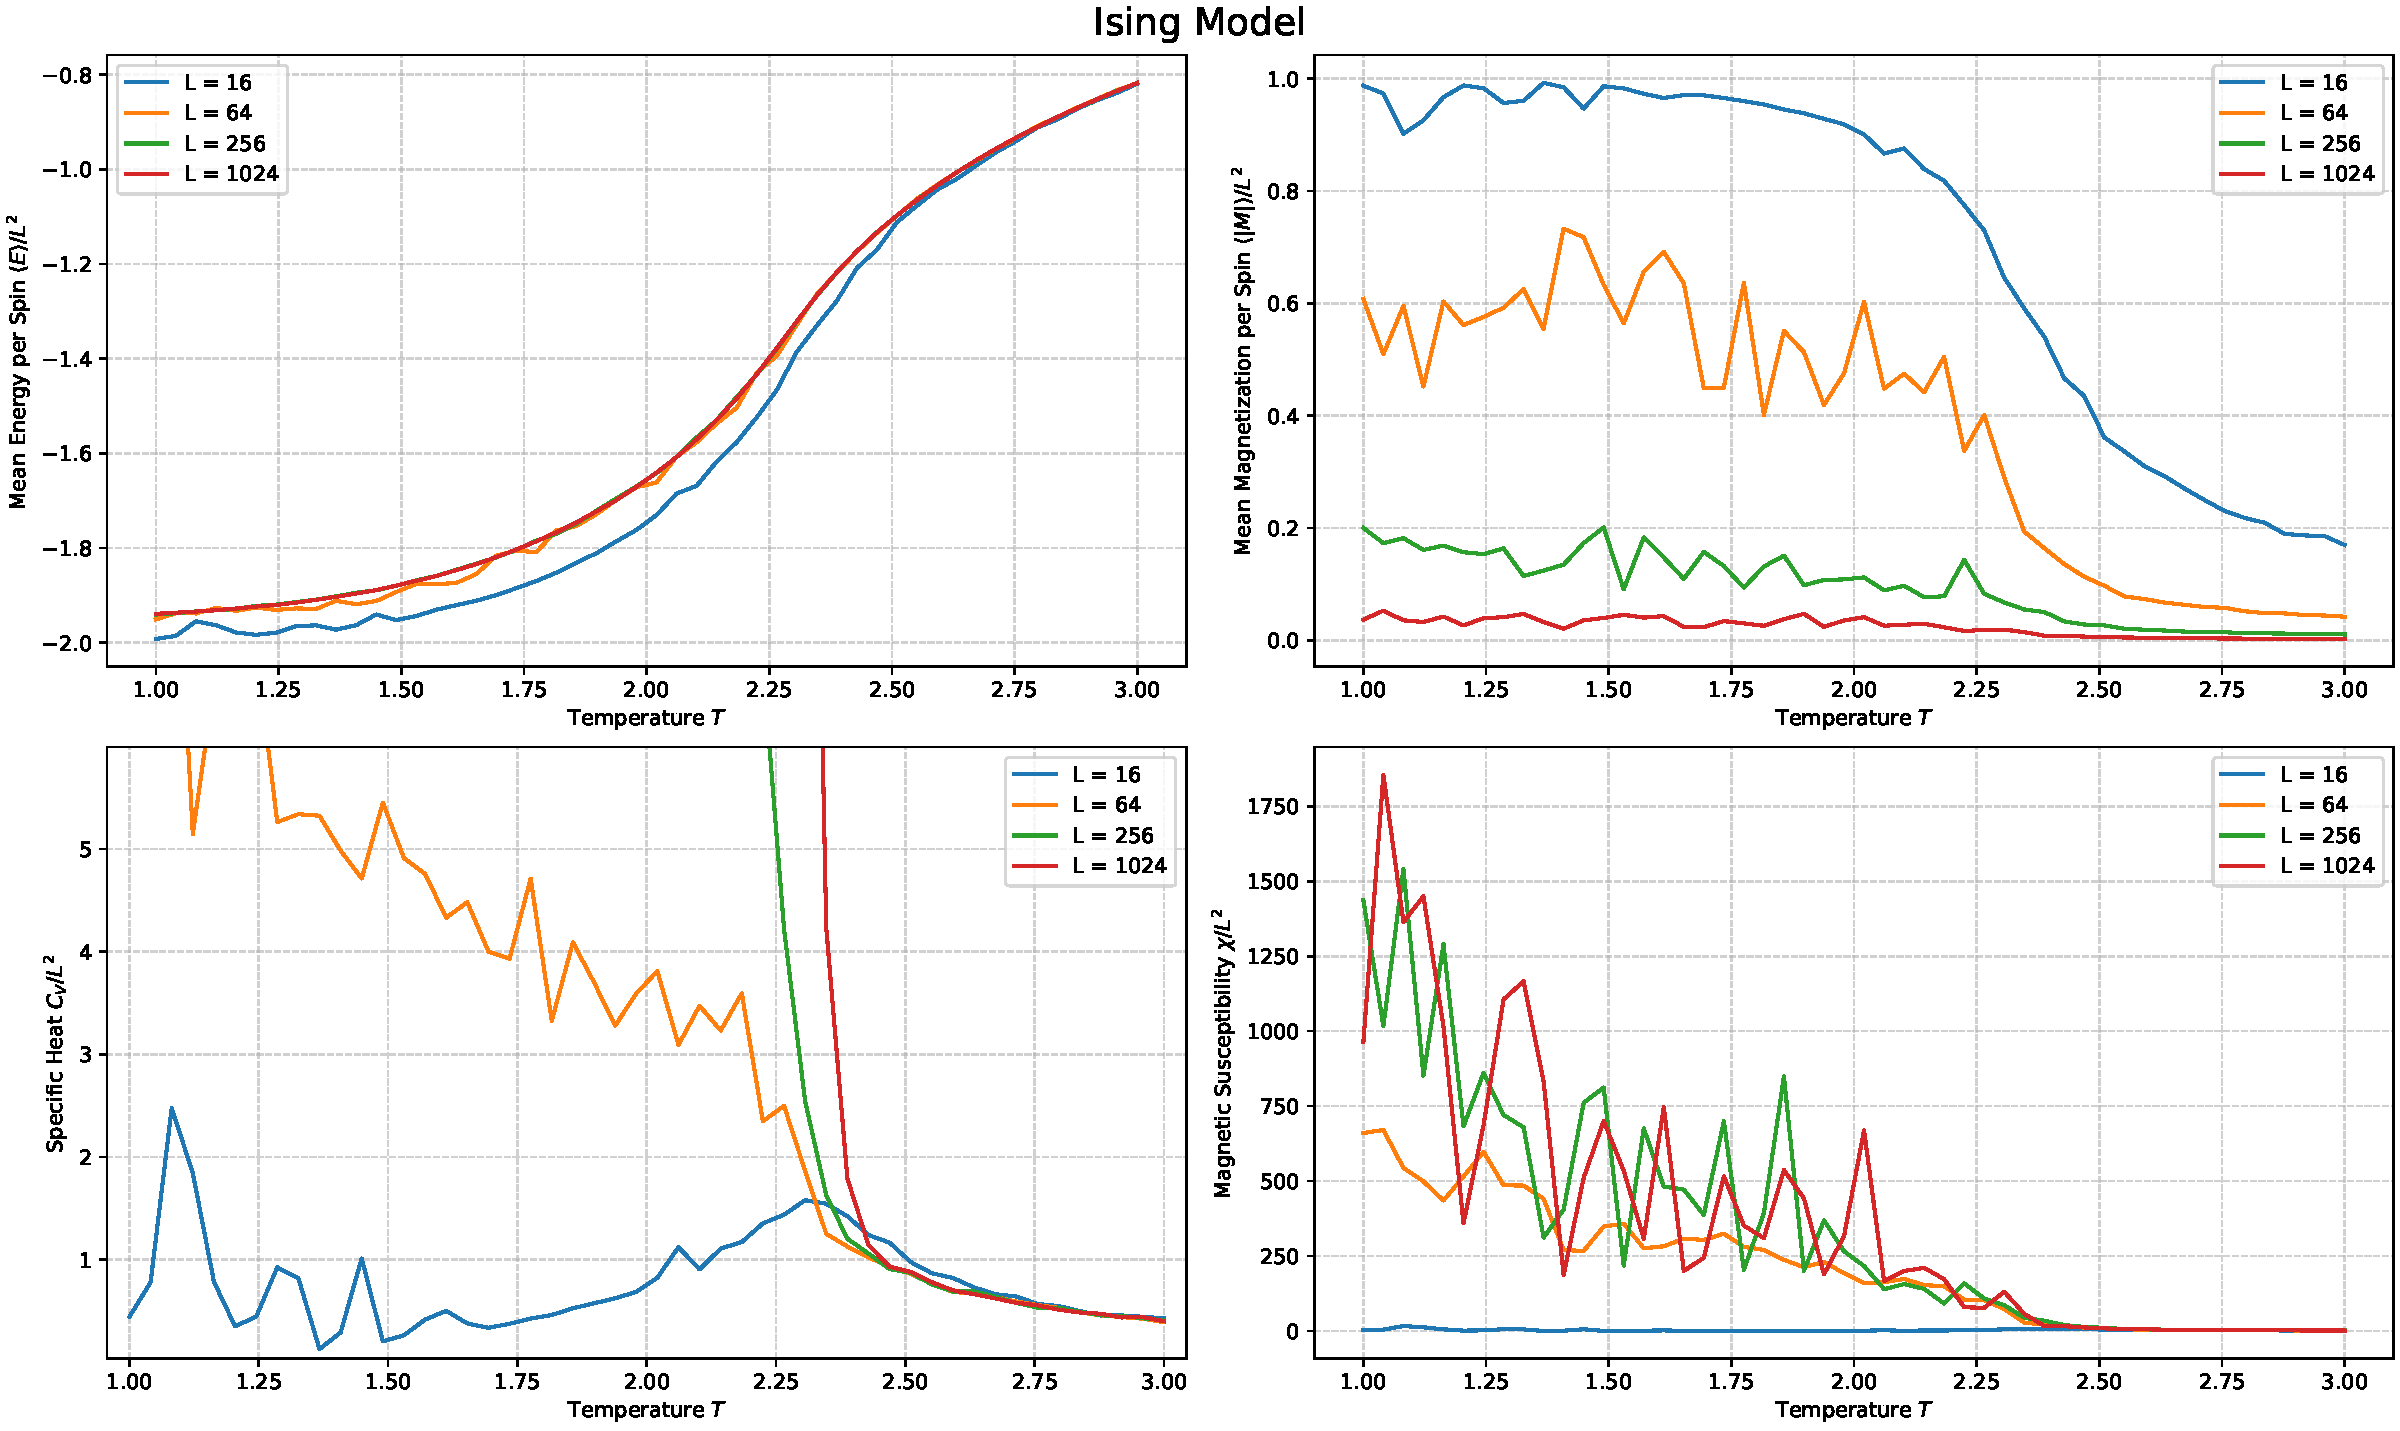
\includegraphics[width=\textwidth]{ising-metropolis.pdf}
  \caption{}
  \label{fig:ising-metropolis}
\end{figure}

\noindent
Further we explore the parallelism of the algorithm using \textit{Amdahls} law. This is shown in figure \ref{fig:ising-metropolis-amdahl}
, yielding a close to one parallelism $p=0.9954$ and inflection point at $n_{inf}=271.1\approx2^{7.76}$\,.
\begin{figure}[h!]
  \centering
  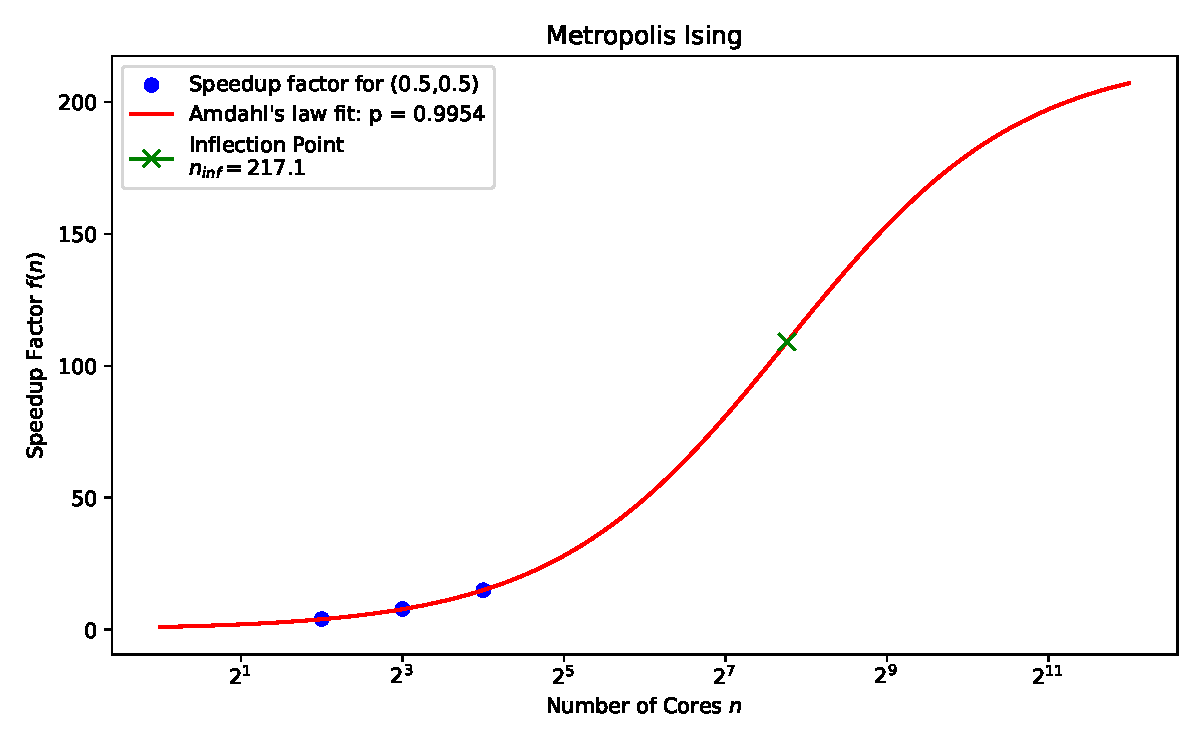
\includegraphics[width=0.7\textwidth]{amdahl-metropolis-ising.pdf}
  \caption{}
  \label{fig:ising-metropolis-amdahl}
\end{figure}


\subsection{Wolff}
To handle larger lattices the Wolff algorithm was implemented, flipping entire clusters.
This also corresponds to a Metropolis walk, however now steps are used to determine the lattice and its size 
to flip. The results of applying this scheme to the Ising model are shown in 
Figure \ref{fig:ising-wolff} for lattices of size $L=16,64,256,1024$\,.
Observe, that now the ordered phase appears as expected, aswell as a peak in 
the specific heat. 
\begin{figure}[h!]
  \centering
  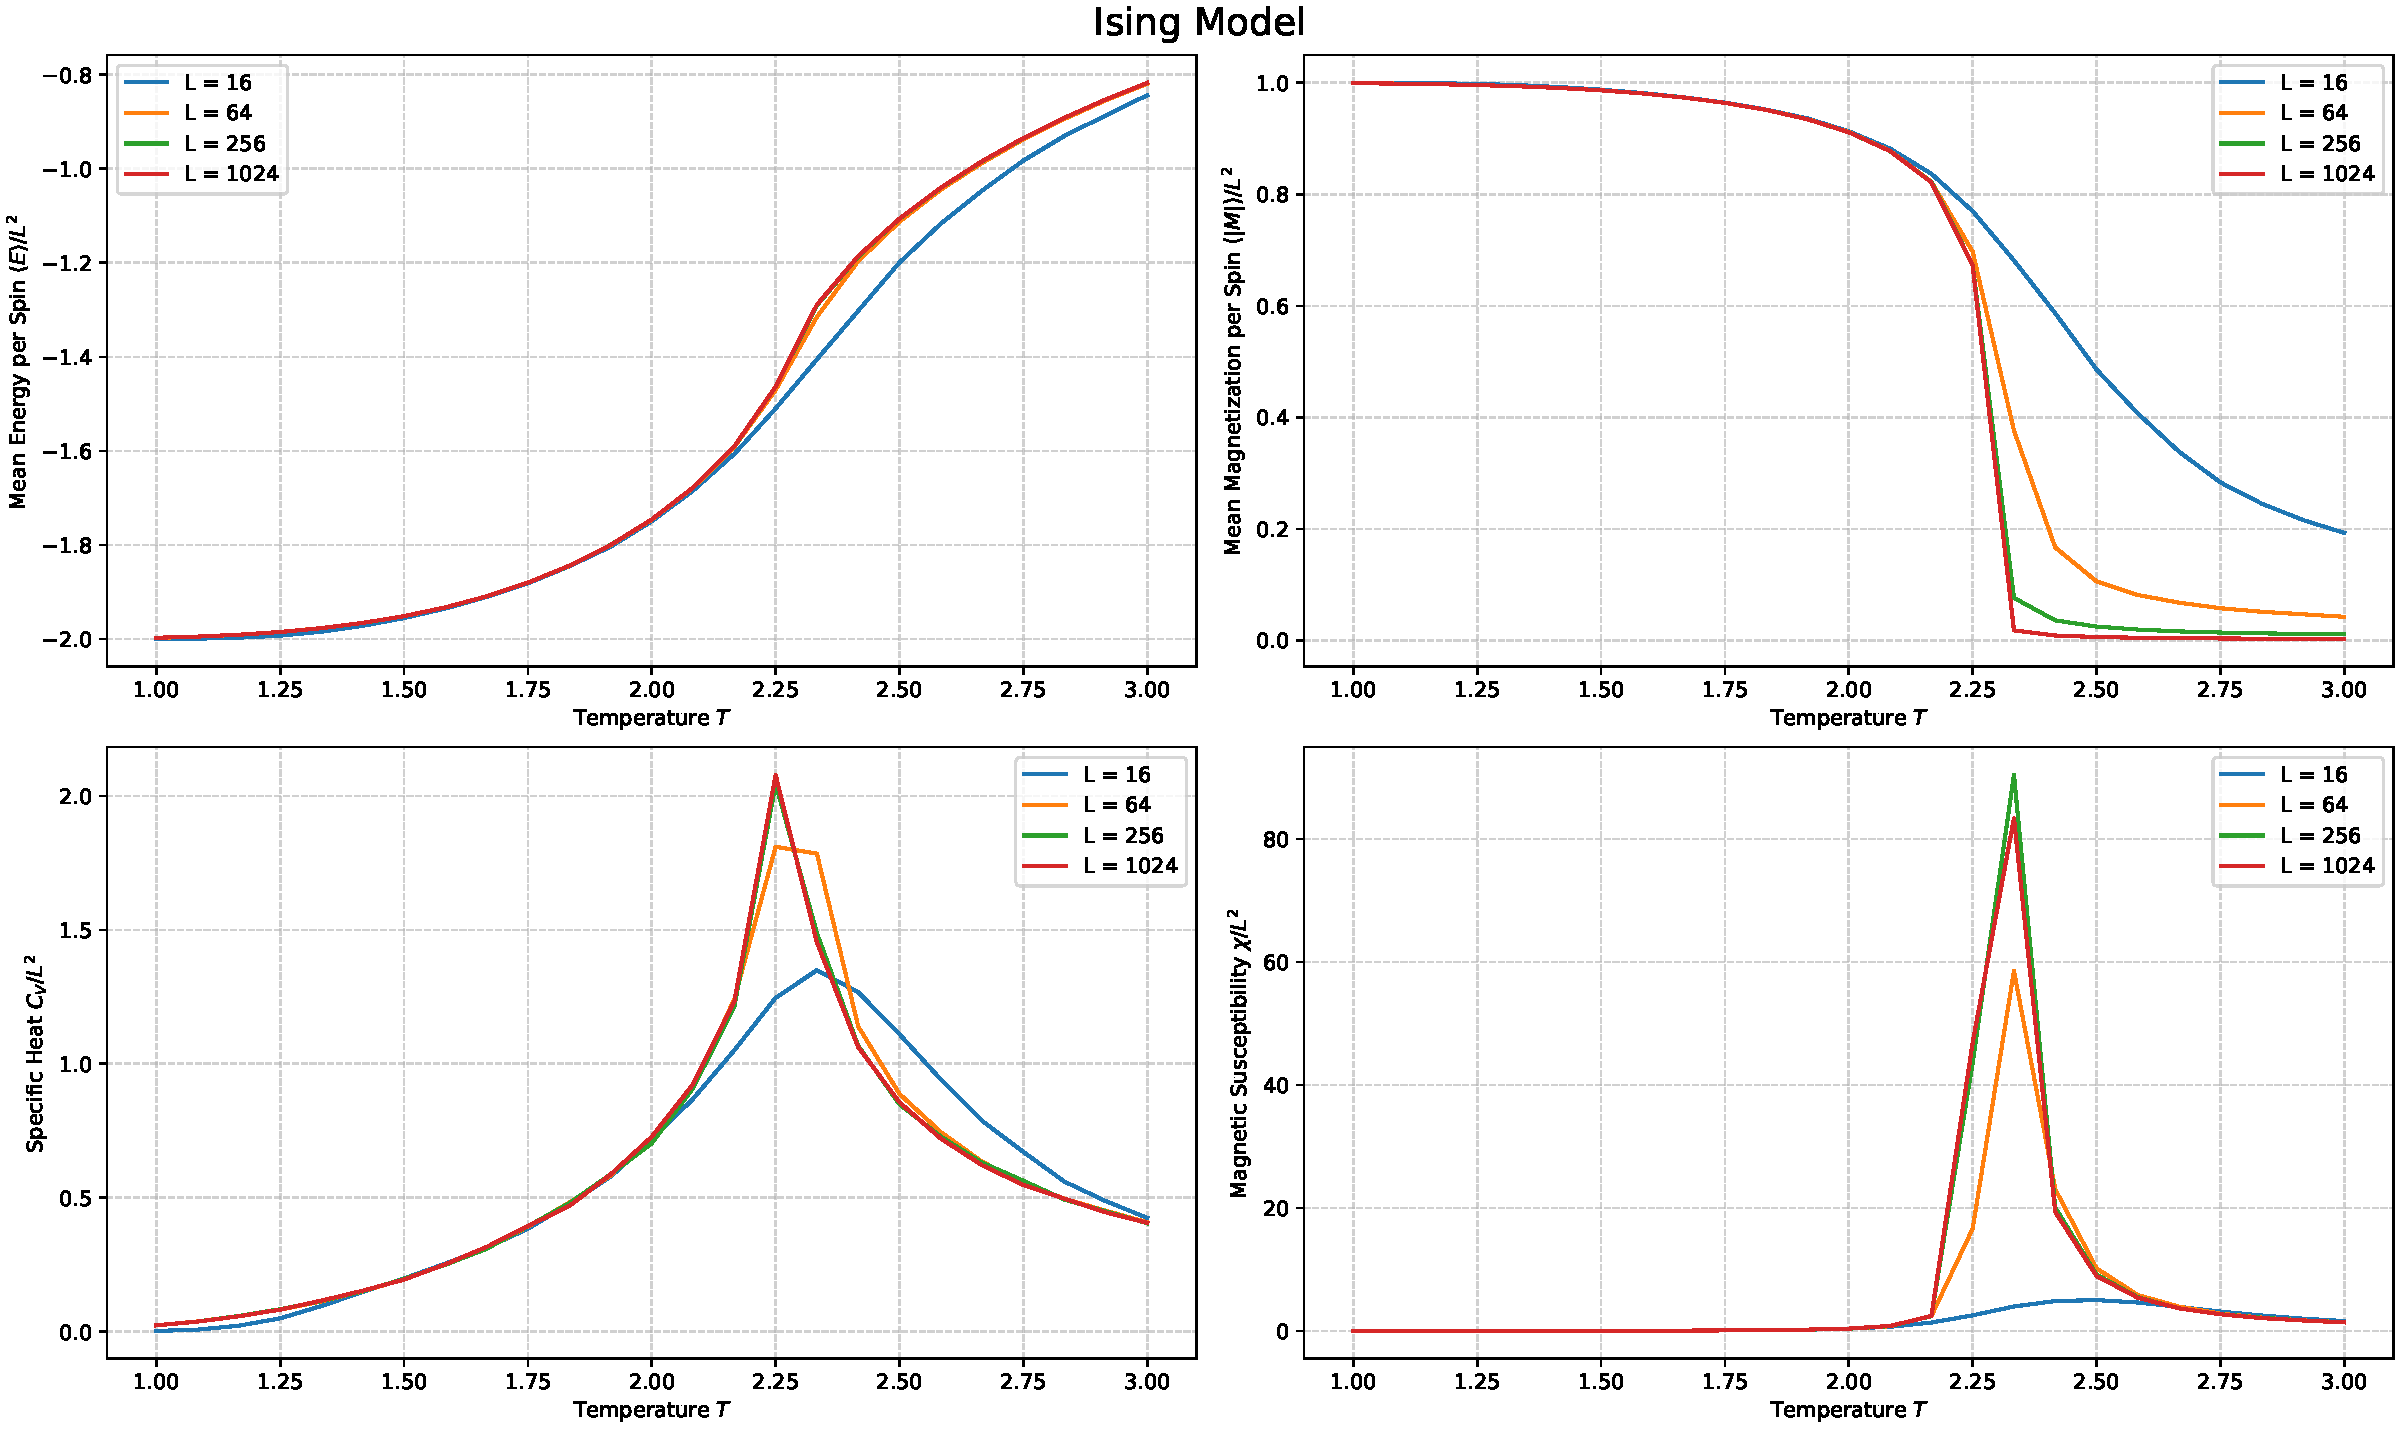
\includegraphics[width=\textwidth]{ising-wolff.pdf}
  \caption{}
  \label{fig:ising-metropolis}
\end{figure}

\noindent
Again \textit{Amdahls} law yields a close to one parallelism $p=0.9957$ and inflection point at $n_{inf}=233.3\approx2^{7.78}$\,.


\section{XY model}
\subsection{Metropolis}
The XY model in two dimensions exhibits a BKT phase transition at $T_c=0.893$\,.
This means that below $T_c$ a ordered phse appears forming vortices. We will see, 
that a quasi long range order appears, given by a power law behavior of correlations.
In the high temperature phase, i.e. disorder, a exponential decay appears.
We still expect a maximum of the specific heat at $T_c$\,.
Results obtained with standard Metropolis are shown in Figure \ref{fig:xy-metropolis}.
\begin{figure}[h!]
  \centering
  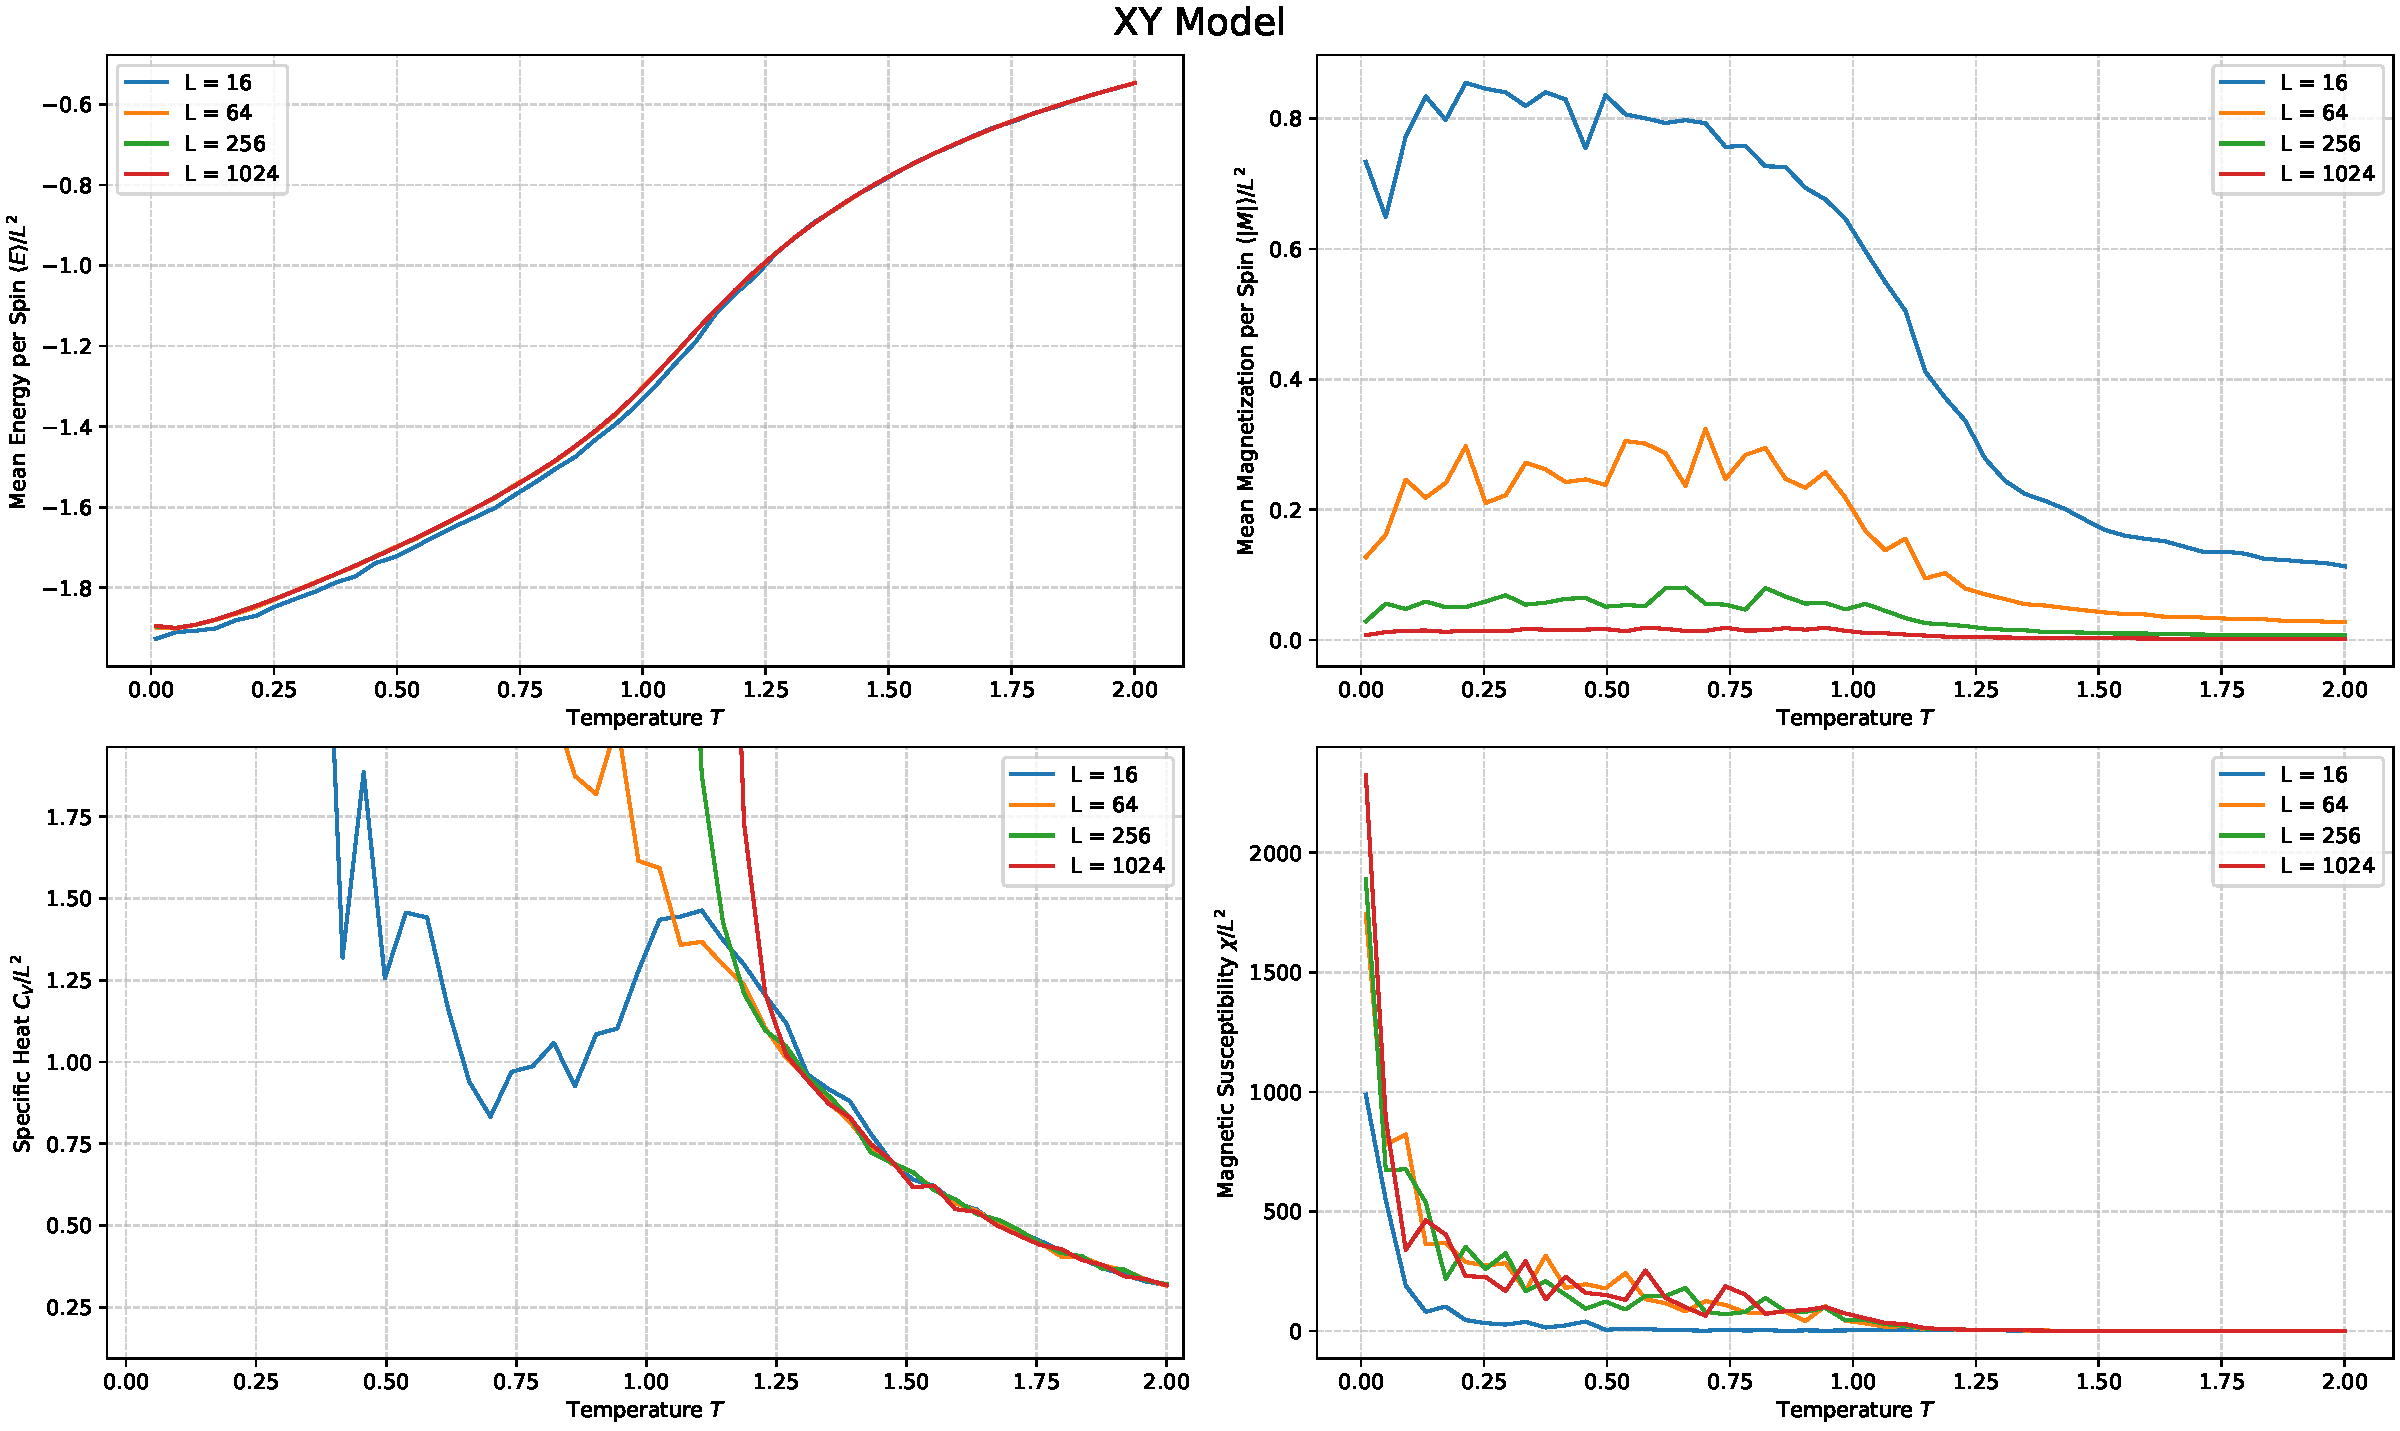
\includegraphics[width=\textwidth]{xy-metropolis.pdf}
  \caption{}
  \label{fig:xy-metropolis}
\end{figure}
Observe, that for $L=16$ the mentioned expectations appear. Beyond that the system 
cannot find its equilibrium state in reasonable time. Note, that the specific heat diverges
due to being energy fluctuations divided by temperature, only saturating if the equilibrium state is found.
\\\\
Again \textit{Amdahls} law yields a close to one parallelism $p=0.9974$ and inflection point at $n_{inf}=382.0\approx2^{8.58}$\,.

\newpage
\subsection{Wolff}
Again a Wolff cluster algorithm was implemented to handle larger lattices. The results
are shown in Figure \ref{fig:xy-wolff}. These match the predictions better.
\begin{figure}[h!]
  \centering
  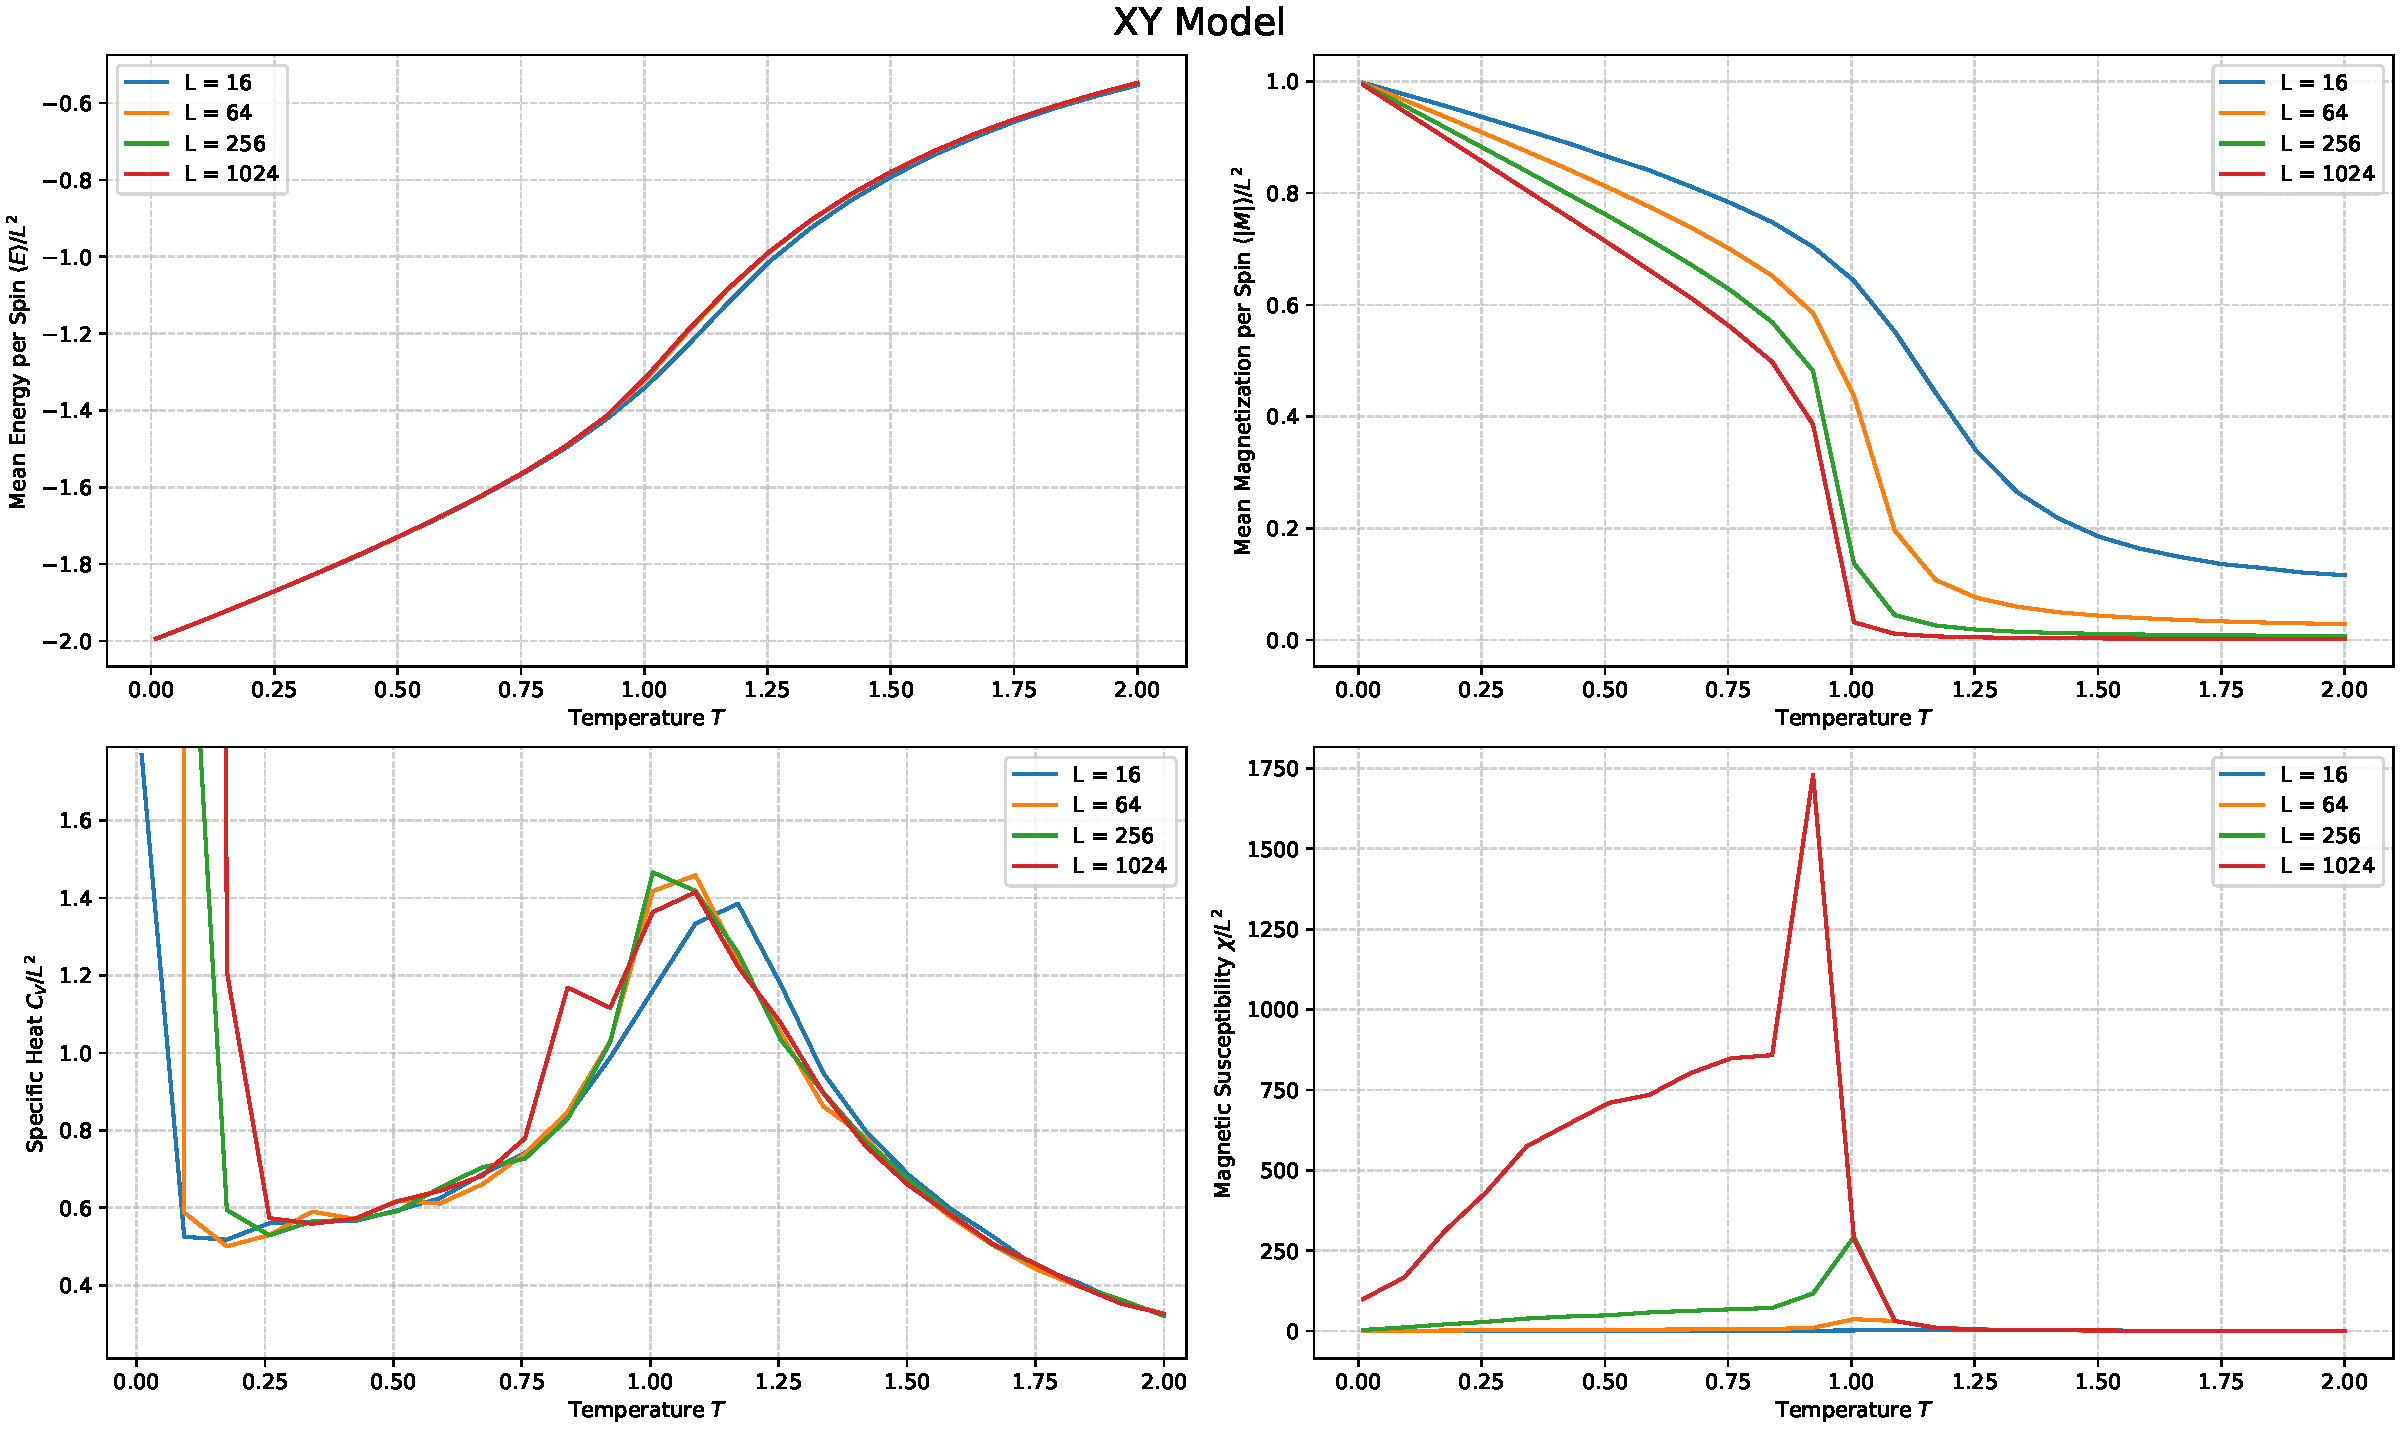
\includegraphics[width=\textwidth]{xy-wolff.pdf}
  \caption{}
  \label{fig:xy-wolff}
\end{figure}

\noindent
Again \textit{Amdahls} law yields a close to one parallelism $p=0.9985$ and inflection point at $n_{inf}=682.0\approx2^{9.4}$\,.


\subsection{Spin Correlations}
We expect a power law behavior below the critical temperature and an exponential decay above. The correlation functions for 
$L=1024$ and $T=0.5,2.0$ are shown in figure \ref{fig:xy-correlations}. 
The better converging Wolff algorithm was used to obtain these correlations.
\begin{figure}[h!]
  \centering
  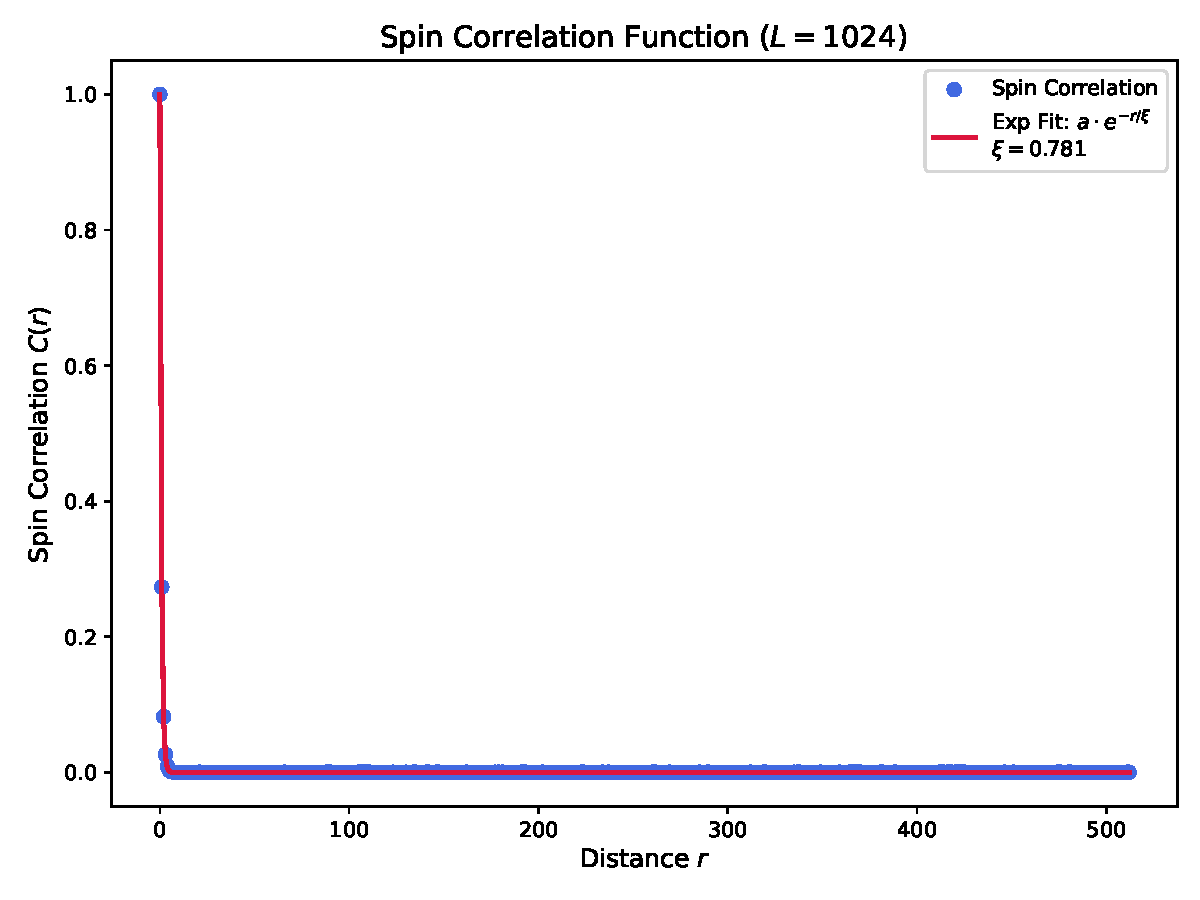
\includegraphics[width=0.48\textwidth]{xy-exp.pdf}
  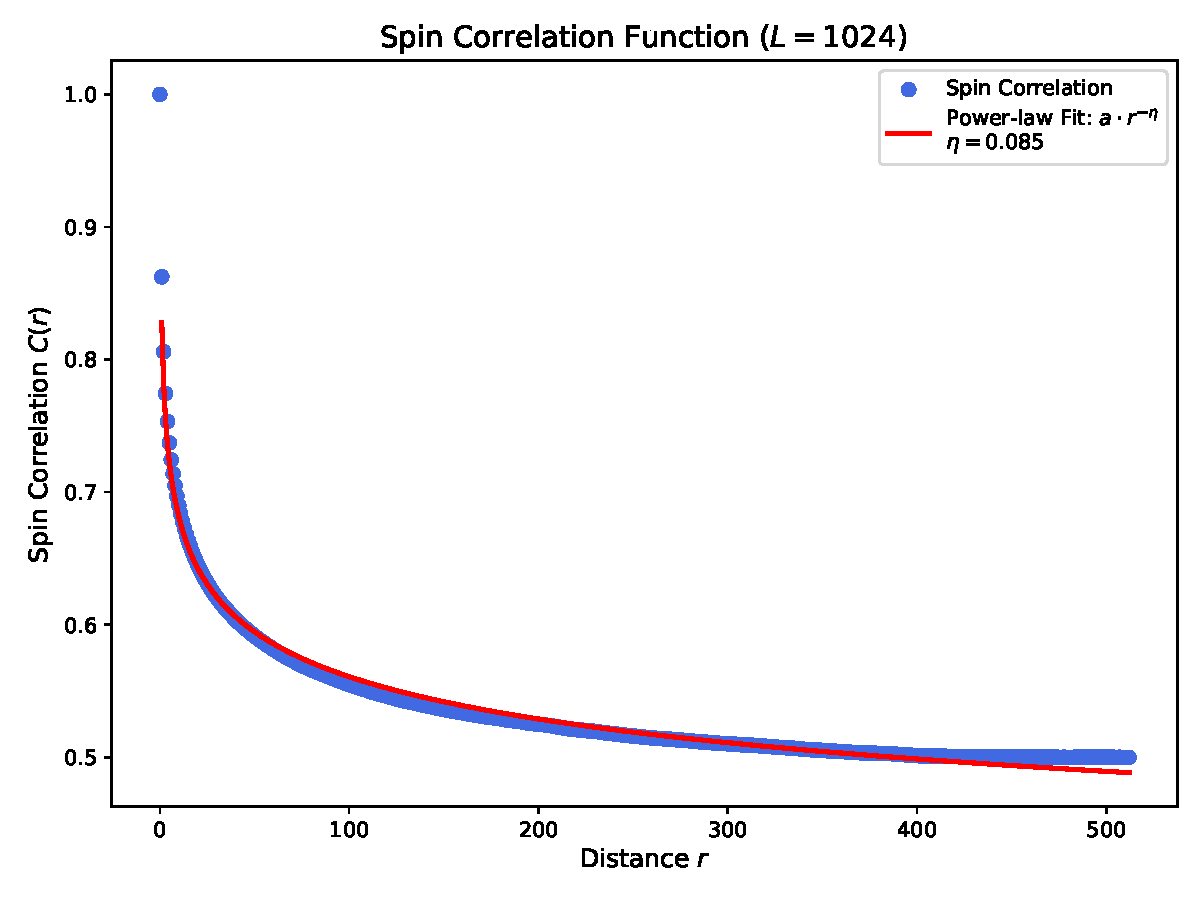
\includegraphics[width=0.48\textwidth]{xy-power.pdf}
  \caption{}
  \label{fig:xy-correlations}
\end{figure}
\\\\
Find the repository under \url{https://github.com/joern16/advanced-computational-physics}.


%----------------------------------------------------------------------------------------
%	BIBLIOGRAPHY
%----------------------------------------------------------------------------------------

%\bibliography{sources}

%----------------------------------------------------------------------------------------
\end{document}